

\section{Empirical Results}


In this section, we will present the results of our empirical study to answer the following research questions: \textbf{(1)} Can training on self-generated trajectories from a diverse range of task groups equip LLMs with sequential decision making capabilities that generalize to unseen task groups without the need to train on them? \textbf{(2)} Can curriculum learning improve the data efficiency of our training mechanism? \textbf{(3)} Finally, does \ours{} hurt the model's regular abilities, and can fine-tuning on existing multiturn interaction data that do not have any sequential decision making structure also improve these capabilities? We first describe our experimental setup, and then report our empirical observations.

\begin{figure*}[h]
    \centering
    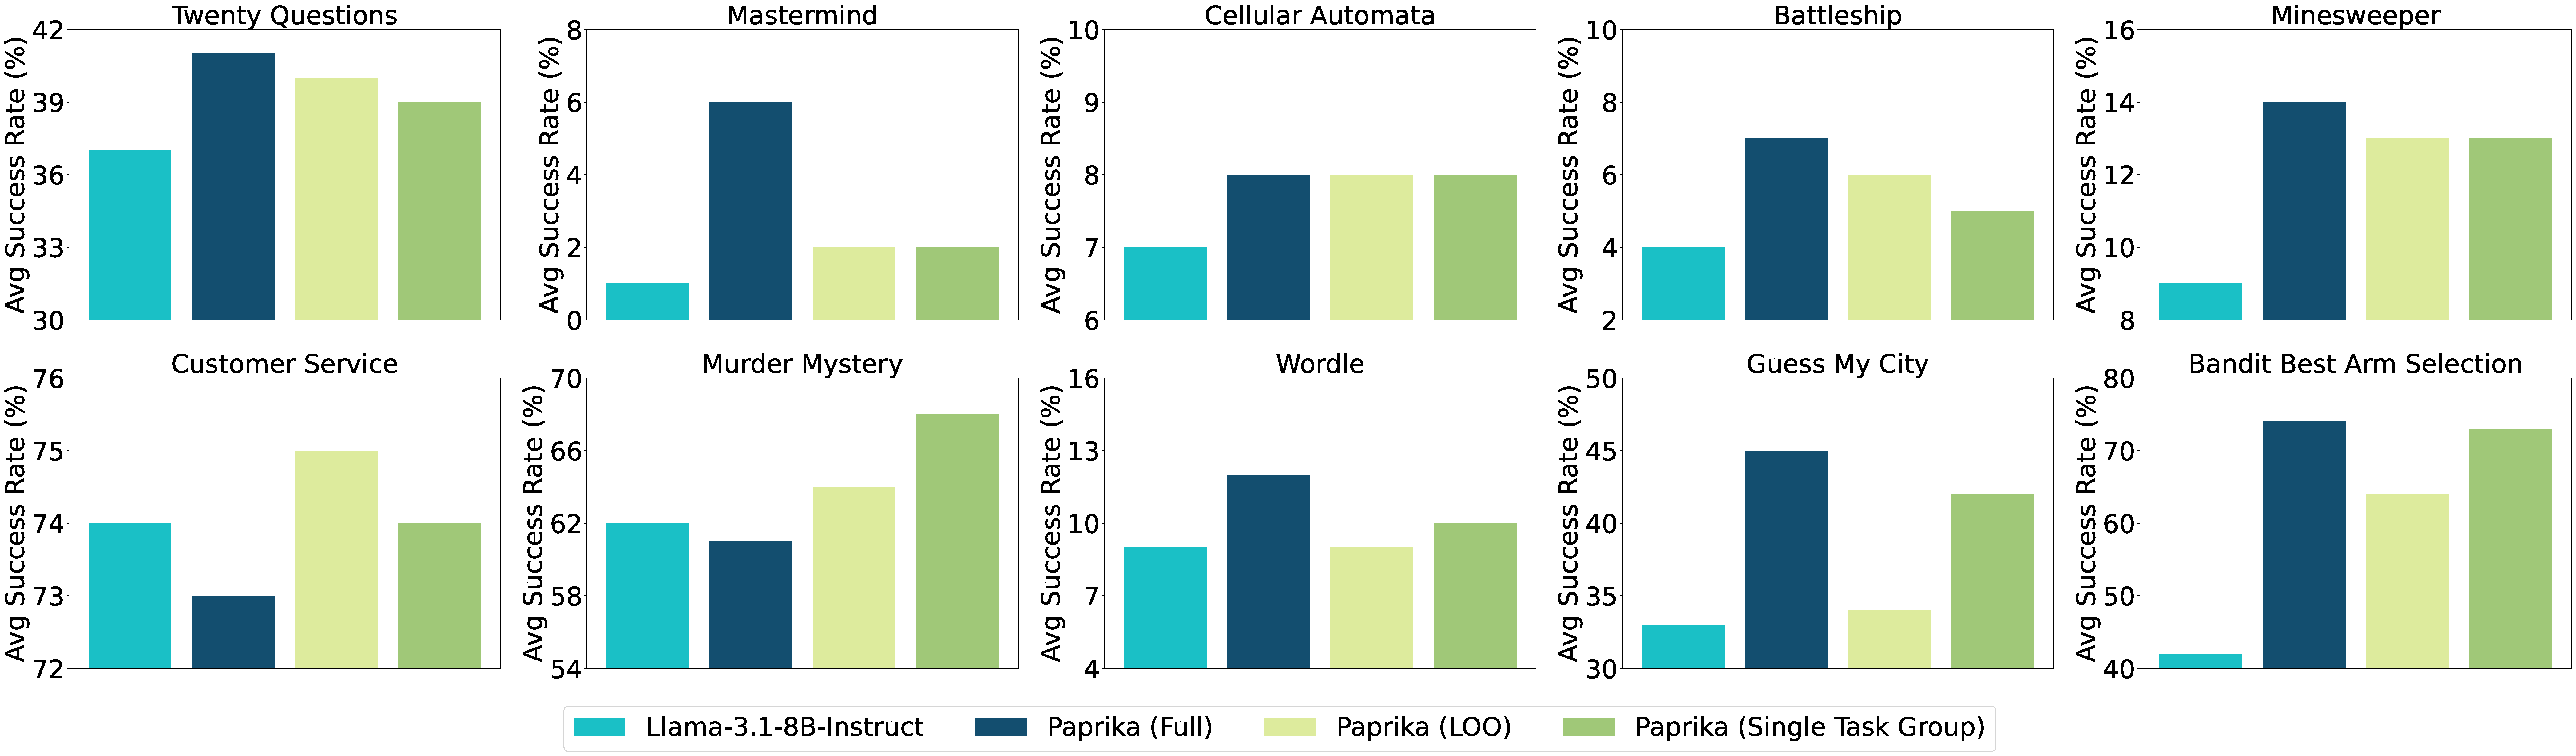
\includegraphics[width=0.99\linewidth]{figures/generalization.pdf}
    \vspace{-0.2cm}
    \caption{\footnotesize \textbf{(Testing generalization of \ours{} via leave-one-out and single task group experiments)} We test \ours{}'s zero-shot performance on unseen task groups by leave-one-out (LOO) experiments, where we train the LLM on every task group except the group we test on. We also report the performance of \ours{} (Single Task Group), where we train and test the LLM on a single group. Our experiments demonstrate that \ours{} can teach an LLM decision making abilities that often transfer well to new tasks without any additional training, and the model also generally learns better in-group strategies when it observes trajectories from other task groups.}
    \label{fig:generalization_leave_one_out_experiments}
    \vspace{-0.2cm}
\end{figure*}

\paragraph{Experimental Setup.}

For experiments in this paper, we use Llama-3.1-8B-Instruct~\citep{grattafiori2024llama3herdmodels} and Gemma-3-12B-IT~\citep{gemmateam2025gemma3technicalreport} models. For data generation, we use Min-p sampling~\citep{nguyen2024turning} with temperature 1.5 and Min-p parameter 0.3, as we saw that this setting consistently generated diverse training data that resulted in higher test-time accuracy. For each task in the training split, we generate $n_\text{sample} = 20$ trajectories to construct our training dataset (except for mastermind, where we sample $n_{\text{sample}} = 100$ trajectories per task). After filtering, this results in 17,181 training trajectories for supervised fine-tuning and 5,260 trajectory pairs for RPO over all task groups. Unless explicitly mentioned otherwise, we use learning rate of $10^{-6}$ for supervised fine-tuning and $2 \times 10^{-7}$ for RPO. We use batch size 32 for all training runs. We generally always run supervised fine-tuning first and then further fine-tune with the RPO objective to obtain the final model unless explicitly mentioned otherwise. We use an AdamW optimizer~\citep{loshchilov2019decoupledweightdecayregularization} with a cosine annealing learning rate scheduler and warmup ratio 0.04~\citep{loshchilov2017sgdrstochasticgradientdescent} to train all our models.

During evaluation, in order to account for variability of both the environment and the agent, we generate 4 trajectories for each task in the test set and report the average success rate (we also report pass@4 success rates in \cref{section:additional_experimental_results}). We use Min-p sampling with parameter 0.3 for evaluation. Default temperature for evaluation is set to 0.7. Finally, for task groups with hardcoded feedback mechanism, we consider a failure to follow formatting instructions to be a failure in the task.


\paragraph{\ours{} improves LLM decision making abilties.}

We motivate this question by looking into the toy task group of bandit best arm selection more closely. This task requires strategic use of the fixed sampling budget (20) to quickly discard arms that are unlikely to have a high mean reward, and use most of the sampling budget on the few top arms to decide the best arm among them. Previous work~\citep{nie2024evolveevaluatingoptimizingllms} has shown that training on synthetic trajectories from optimal bandit algorithms can significantly improve LLMs' performance on them. Contrary to that, we show that LLMs can learn generalizable strategies from other decision making task groups that then transfer to this bandit group, without needing an optimal algorithm to generate synthetic trajectories. \cref{fig:generalization_leave_one_out_experiments} shows that \ours{} improves average success rate of Llama-3.1-8B-Instruct from 42.25\% to 62.25\% on the bandit task after only seeing trajectories from other task groups.

Motivated by this, we next study whether \ours{} can also improve performance on more complex tasks. \cref{fig:paprika_success_rate} shows our main findings: \ours{}, when trained on a dataset consisting of filtered trajectories from all 10 task groups, improves the success rate of both Llama-3.1-8B-Instruct and Gemma-3-12B-It models (see \cref{section:additional_experimental_results} for complete results).
Averaged across all 10 task groups, \ours{} increases the Llama-3.1-8B-Instruct model's performance by 47\% of its original success rate after training with only about 22,500 trajectories.

\paragraph{\ours{} can teach LLMs generalizable strategies.}

The next important question we want to study is whether the strategies learned by \ours{} can zero-shot transfer to entirely different groups of tasks. We saw already that \ours{} (LOO) improved the success rate on the bandit group without the need to train on it, now we explore this possibility for more complex decision making tasks. To do so, we perform a set of leave-one-out (LOO) experiments: we randomly choose one group (e.g., 20 questions) from our set of task groups, train the LLM on trajectories generated from every other group, and test the resulting model's performance on the left-out group. 
Additionally, we run an experiment where for each task group, we train and test the LLM on only this single group (using separate splits). We use Llama-3.1-8B-Instruct for this set of experiments.

\cref{fig:generalization_leave_one_out_experiments} shows our results: remarkably, we observe that the LOO models can match or sometimes even exceed the performance of group-specific training, demonstrating genuine cross-task group generalization. Concretely, \ours{} (LOO) improves success rate on 9 out of 10 task groups compared to the initial model. Moreover, \ours{} (full), trained on all 10 task groups, outperform \ours{} (Single Task Group) in 7 out of 10 task groups, showing that the model learns better in-group strategies when it observes trajectories from other task groups. Note that we do not expect \ours{} (LOO) to always generalize to a new task group. While \ours{} (LOO) generalizes better to some task groups vs others (e.g., the improvement on mastermind is minimal), and for some task groups there is no transfer at all or negative transfer (wordle), we hypothesize that scaling up the number of task groups could keep improving LLMs' zero-shot decision-making abilities. Overall, these results demonstrate that \ours{} is a potentially scalable solution for teaching LLMs how to do in-context RL.

\begin{figure*}[h]
    \centering
    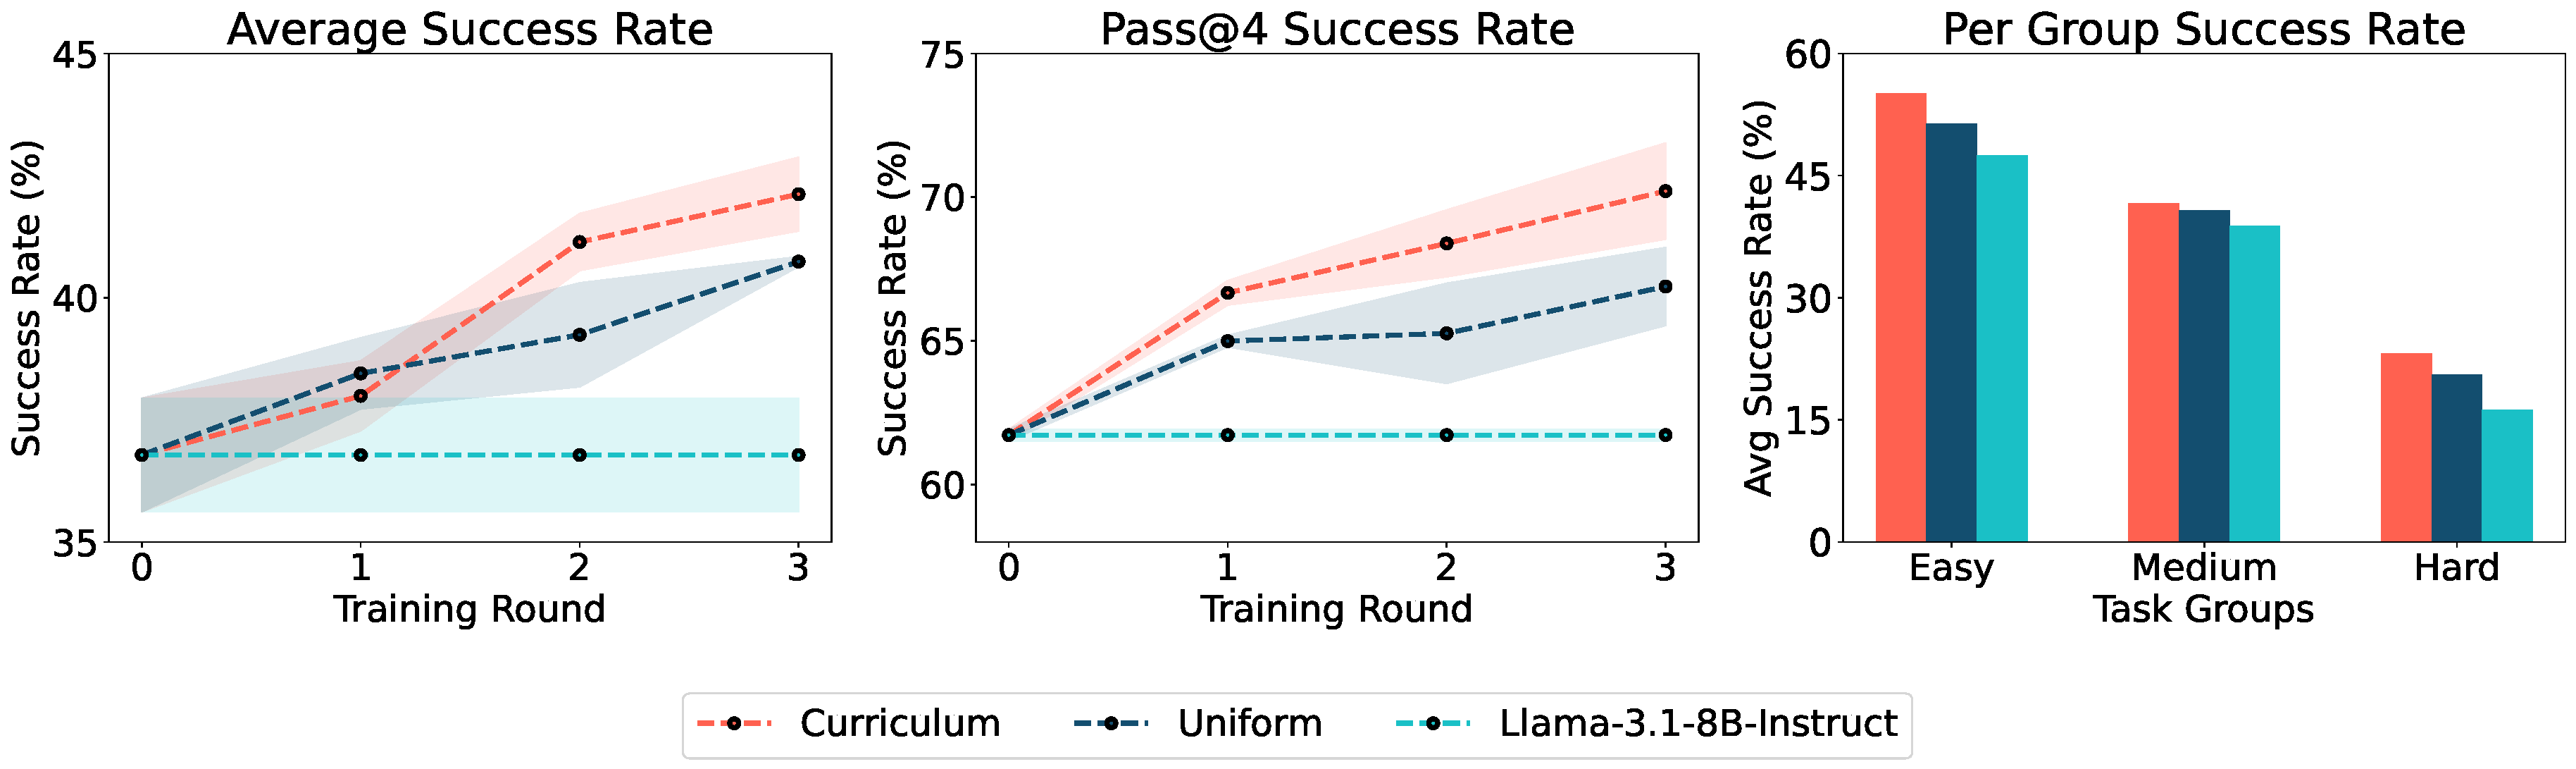
\includegraphics[width=0.99\linewidth]{figures/curriculum.pdf}
    \vspace{-0.3cm}
    \caption{\footnotesize \textbf{(Multi-round training with curriculum on twenty questions)} We demonstrate the efficacy of our curriculum learning algorithm for sampling training tasks by comparing its performance against uniform sampling for multi-round training. All experiments use Llama-3.1-8B-Instruct as the initial model, evaluations are done at temperature 0.7, and shaded regions represent standard error over 3 seeds. (\textbf{Left}) Average success rate at each round. (\textbf{Middle}) Pass@4 success rate at each round. (\textbf{Right}) Success rate per each of easy, medium, and hard task groups. Overall, our curriculum learning algorithm shows 1.4\% and 3.3\% improvement over the uniform sampling baseline at average and pass@4 success rate respectively.}
    \label{fig:curriculum}
    \vspace{-0.35cm}
\end{figure*}


\paragraph{Curriculum learning can improve data efficiency of \ours{}.}



The biggest bottleneck of \ours{} is the time required to generate a large number of trajectories for each. 
Some tasks are naturally harder than others, which means that spending an equal sampling budget on the harder tasks gives us a smaller learning signal. 
We study a curriculum learning version of \ours{} where we have a grouping over our tasks according to task difficulty. For this, we use GPT-4o-mini to classify the tasks in twenty questions into 3 categories: easy, medium, and hard. This results in 477 easy, 726 medium, and 296 hard topics in the train split and 127 easy, 172 medium, and 68 hard topics in the test split. 

Next, we run the curriculum learning algorithm described in \cref{section:curriculum} for 3 rounds on a Llama-3.1-8B-Instruct model: at each round, we sample 250 tasks from the train set according to \cref{alg:sampling}. We use the number of turns it took the agent to solve a task across multiple trajectories as a proxy for reward in \cref{eq:nu} to calculate $\nu_{\pi}$ (see \cref{appendix:curriculum} for more details). 20 trajectories are generated for each task using the previous round's model checkpoint and we train that checkpoint on the resulting dataset (for DPO, we use the prior round's checkpoint instead of the initial model as the reference policy). We compare our curriculum against the baseline of sampling 250 tasks uniformly at random from the train set at each round. \cref{fig:curriculum} shows our results: after three rounds of training, our curriculum outperforms uniform sampling by 1.4\% and 3.3\% at average and pass@4 accuracy respectively.


\subsection{Analysis}


\paragraph{\ours{} improves LLMs' task efficiency.} In this section, we want to analyze the sequential decision-making abilities learned by \ours{} beyond just success rate on individual task groups. Note that our tasks are designed in a way such that an agent capable of better strategic exploration would solve them faster, eg., an agent capable of asking better yes/no questions would guess the secret topic using fewer number of turns. We leverage this property of our tasks and conduct both quantitative and qualitative analysis on the behaviors of the regular instruct model and \ours{} --- \textbf{(1)} \cref{fig:all_environment_temperature_ablation_num_turns} shows that \ours{} reduces the average number of turns it takes for the agent to solve tasks, implying that \ours{} is choosing more optimal actions at intermediate steps,  \textbf{(2)} \cref{appendixSection:example_trajectories} shows qualitative difference between the behavior of the regular instruct model and \ours{} on twenty questions and wordle, with \ours{} generally generating more sensible responses.

\begin{table*}
    \centering
        \caption{\footnotesize \textbf{(Evaluation of \ours{} on standard tasks)} Evaluation of \ours{} vs Llama-3.1-8B-Instruct on standard benchmarks (numbers in parenthesis represent standard error over 3 seeds). \ours{} does not result in significant model degradation.}
        \vspace{0.2cm}
        \begin{tabular}{c|cccccc}
            \toprule
            Model & MT-Bench & AlpacaEval & GPQA & Math (Hard) & MMLU-Pro & IFEval \\
            \midrule
             Llama-3.1-8B-Instruct & 7.88 & \textbf{33.6} & \textbf{33.5} & 24.6 & \textbf{46.7} & 84.4\\
             + \ours{} & \textbf{8.14 (0.03)} & 33.5 (0.3) & 32.8 (1.5) & \textbf{25.3 (0.3)} & 46.2 (0.1) & \textbf{85.4 (0.3)} \\
             \bottomrule
        \end{tabular}
    \vspace{-0.2cm}
    \label{tab:mt_bench_eval}
\end{table*}

\paragraph{\ours{} does not hurt LLMs' regular capabilities.} We have demonstrated the efficacy of \ours{} in instilling decision making capabilities into LLMs efficiently. However, to scale up \ours{}, one would potentially use online reinforcement learning on such decision making tasks, and an important question is whether \ours{} fine-tuning would hurt the LLM's regular capabilities which would hinder scaling it up. To study this question, we run a set of standard evaluations (see \cref{appendix:standard_evaluations}) on our \ours{} fine-tuned model and compare its performance against Llama-3.1-8B-Instruct. \cref{tab:mt_bench_eval} shows our findings: \ours{} does not result in any noticeable performance degradation.
